% Options for packages loaded elsewhere
\PassOptionsToPackage{unicode}{hyperref}
\PassOptionsToPackage{hyphens}{url}
\PassOptionsToPackage{dvipsnames,svgnames,x11names}{xcolor}
%
\documentclass[
]{estat/estat}

\usepackage{amsmath,amssymb}
\usepackage{iftex}
\ifPDFTeX
  \usepackage[T1]{fontenc}
  \usepackage[utf8]{inputenc}
  \usepackage{textcomp} % provide euro and other symbols
\else % if luatex or xetex
  \usepackage{unicode-math}
  \defaultfontfeatures{Scale=MatchLowercase}
  \defaultfontfeatures[\rmfamily]{Ligatures=TeX,Scale=1}
\fi
\usepackage{lmodern}
\ifPDFTeX\else  
    % xetex/luatex font selection
    \setmainfont[]{Arial}
\fi
% Use upquote if available, for straight quotes in verbatim environments
\IfFileExists{upquote.sty}{\usepackage{upquote}}{}
\IfFileExists{microtype.sty}{% use microtype if available
  \usepackage[]{microtype}
  \UseMicrotypeSet[protrusion]{basicmath} % disable protrusion for tt fonts
}{}
\makeatletter
\@ifundefined{KOMAClassName}{% if non-KOMA class
  \IfFileExists{parskip.sty}{%
    \usepackage{parskip}
  }{% else
    \setlength{\parindent}{0pt}
    \setlength{\parskip}{6pt plus 2pt minus 1pt}}
}{% if KOMA class
  \KOMAoptions{parskip=half}}
\makeatother
\usepackage{xcolor}
\usepackage[left=3cm,right=2cm,top=3cm,bottom=2cm]{geometry}
\setlength{\emergencystretch}{3em} % prevent overfull lines
\setcounter{secnumdepth}{5}
% Make \paragraph and \subparagraph free-standing
\makeatletter
\ifx\paragraph\undefined\else
  \let\oldparagraph\paragraph
  \renewcommand{\paragraph}{
    \@ifstar
      \xxxParagraphStar
      \xxxParagraphNoStar
  }
  \newcommand{\xxxParagraphStar}[1]{\oldparagraph*{#1}\mbox{}}
  \newcommand{\xxxParagraphNoStar}[1]{\oldparagraph{#1}\mbox{}}
\fi
\ifx\subparagraph\undefined\else
  \let\oldsubparagraph\subparagraph
  \renewcommand{\subparagraph}{
    \@ifstar
      \xxxSubParagraphStar
      \xxxSubParagraphNoStar
  }
  \newcommand{\xxxSubParagraphStar}[1]{\oldsubparagraph*{#1}\mbox{}}
  \newcommand{\xxxSubParagraphNoStar}[1]{\oldsubparagraph{#1}\mbox{}}
\fi
\makeatother


\providecommand{\tightlist}{%
  \setlength{\itemsep}{0pt}\setlength{\parskip}{0pt}}\usepackage{longtable,booktabs,array}
\usepackage{calc} % for calculating minipage widths
% Correct order of tables after \paragraph or \subparagraph
\usepackage{etoolbox}
\makeatletter
\patchcmd\longtable{\par}{\if@noskipsec\mbox{}\fi\par}{}{}
\makeatother
% Allow footnotes in longtable head/foot
\IfFileExists{footnotehyper.sty}{\usepackage{footnotehyper}}{\usepackage{footnote}}
\makesavenoteenv{longtable}
\usepackage{graphicx}
\makeatletter
\def\maxwidth{\ifdim\Gin@nat@width>\linewidth\linewidth\else\Gin@nat@width\fi}
\def\maxheight{\ifdim\Gin@nat@height>\textheight\textheight\else\Gin@nat@height\fi}
\makeatother
% Scale images if necessary, so that they will not overflow the page
% margins by default, and it is still possible to overwrite the defaults
% using explicit options in \includegraphics[width, height, ...]{}
\setkeys{Gin}{width=\maxwidth,height=\maxheight,keepaspectratio}
% Set default figure placement to htbp
\makeatletter
\def\fps@figure{htbp}
\makeatother

\authors{%
    Estatiano 1 \\
    Estatiano 2\\
    Estatiano 3\\
}

% escreva o nome do cliente aqui
% se for mais de um separe por \\
\client{%
    ESTAT
}
% Baixando pacotes
\RequirePackage{fancyhdr}
\RequirePackage{graphicx}

\setlength\headheight{28pt}  

\setlength{\parindent}{15pt} % Adiciona indentação nos parágrafos
\setlength{\parskip}{0pt} % Adiciona 0 espaço entro os parágrafos

\let\oldsection\section
\renewcommand\section{\clearpage\oldsection}
\makeatletter
\@ifpackageloaded{float}{}{\usepackage{float}}
\floatstyle{plain}
\@ifundefined{c@chapter}{\newfloat{quadro}{h}{loquad}}{\newfloat{quadro}{h}{loquad}[chapter]}
\floatname{quadro}{Quadro}
\floatstyle{plaintop}
\restylefloat{quadro}
\newcommand*\listofquadros{\listof{quadro}{List of Testes}}
\makeatother
\makeatletter
\@ifpackageloaded{caption}{}{\usepackage{caption}}
\AtBeginDocument{%
\ifdefined\contentsname
  \renewcommand*\contentsname{Índice}
\else
  \newcommand\contentsname{Índice}
\fi
\ifdefined\listfigurename
  \renewcommand*\listfigurename{Lista de Figuras}
\else
  \newcommand\listfigurename{Lista de Figuras}
\fi
\ifdefined\listtablename
  \renewcommand*\listtablename{Lista de Tabelas}
\else
  \newcommand\listtablename{Lista de Tabelas}
\fi
\ifdefined\figurename
  \renewcommand*\figurename{Figura}
\else
  \newcommand\figurename{Figura}
\fi
\ifdefined\tablename
  \renewcommand*\tablename{Tabela}
\else
  \newcommand\tablename{Tabela}
\fi
}
\@ifpackageloaded{float}{}{\usepackage{float}}
\floatstyle{ruled}
\@ifundefined{c@chapter}{\newfloat{codelisting}{h}{lop}}{\newfloat{codelisting}{h}{lop}[chapter]}
\floatname{codelisting}{Listagem}
\newcommand*\listoflistings{\listof{codelisting}{Lista de Listagens}}
\captionsetup{labelsep=colon}
\makeatother
\makeatletter
\makeatother
\makeatletter
\@ifpackageloaded{caption}{}{\usepackage{caption}}
\@ifpackageloaded{subcaption}{}{\usepackage{subcaption}}
\makeatother

\ifLuaTeX
\usepackage[bidi=basic]{babel}
\else
\usepackage[bidi=default]{babel}
\fi
\babelprovide[main,import]{portuguese}
\ifPDFTeX
\else
\babelfont{rm}[]{Arial}
\fi
% get rid of language-specific shorthands (see #6817):
\let\LanguageShortHands\languageshorthands
\def\languageshorthands#1{}
\ifLuaTeX
  \usepackage{selnolig}  % disable illegal ligatures
\fi
\usepackage{bookmark}

\IfFileExists{xurl.sty}{\usepackage{xurl}}{} % add URL line breaks if available
\urlstyle{same} % disable monospaced font for URLs
\hypersetup{
  pdflang={pt},
  colorlinks=true,
  linkcolor={black},
  filecolor={black},
  citecolor={black},
  urlcolor={black},
  pdfcreator={LaTeX via pandoc}}


\author{}
\date{}

\begin{document}

% Limpando tudo
\fancyhf{} 

% Ajustes do header
\fancyhead[L]{} % limpando o lado esquerdo
\fancyhead[R]{\includegraphics[width=0.20\textwidth]{estat/imagens/estat.png}} % adicionando logo no canto direito
\renewcommand{\headrulewidth}{0pt}   % sem linha embaixo da logo

% Ajustes de fim de página
\fancyfoot[R]{\textcolor{white}{\thepage}} % Número em branco no canto direito

% Aplicando o estilo que acabamos de criar
\pagestyle{fancy} 


\labelformat{quadro}{\textbf{#1}}

\renewcommand*\contentsname{Sumário}
{
\hypersetup{linkcolor=}
\setcounter{tocdepth}{3}
\tableofcontents
}

\begin{verbatim}
[1] "C:/Users/Alex Sovat/Documents/PS - ESTAT/Projeto-Fantasma-2026.1"
\end{verbatim}

\begin{verbatim}
pacote 'xlsx' desempacotado com sucesso e somas MD5 verificadas

Os pacotes binários baixados estão em
    C:\Users\Alex Sovat\AppData\Local\Temp\RtmpwtTuKN\downloaded_packages
\end{verbatim}

\begin{verbatim}
# A tibble: 12 x 2
   mes       total_receita_usd
   <ord>                 <dbl>
 1 janeiro                39.1
 2 fevereiro              48.9
 3 março                  44.1
 4 abril                  39.1
 5 maio                   25.6
 6 junho                  62.4
 7 julho                  47.8
 8 agosto                147. 
 9 setembro              332. 
10 outubro               320. 
11 novembro              317. 
12 dezembro              215. 
\end{verbatim}

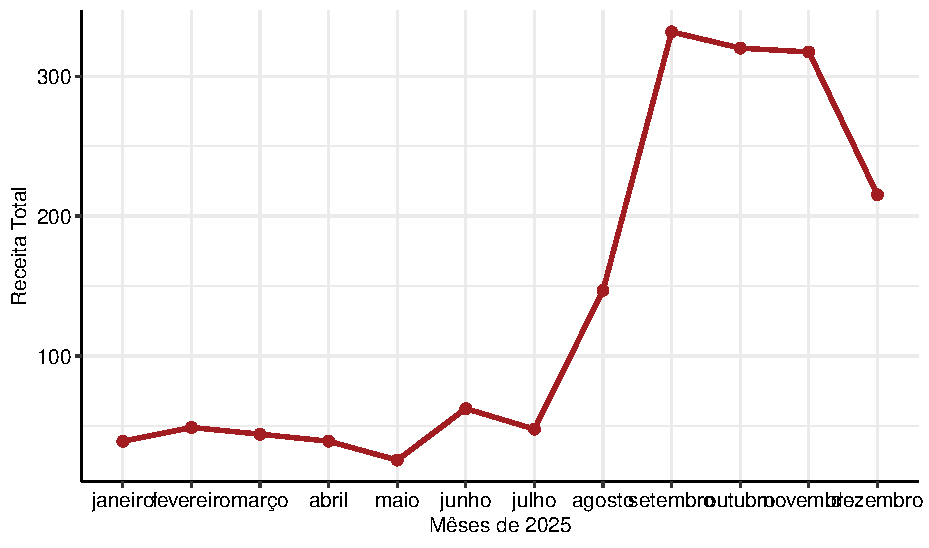
\includegraphics{entrega2_files/figure-pdf/setup-1.pdf}

\begin{verbatim}
\begin{quadro}[H]
    \setlength{ \tabcolsep}{9pt}
    \renewcommand{  \arraystretch}{1.20}
    \caption{Medidas resumo da(o) [nome da variável]}
    \centering
    \begin{adjustbox}{max width=\textwidth}
    \begin{tabular} { | l |
            S[table-format = -Inf.2]
            |}
    \hline
        \textbf{Estatística} & \textbf{Valor} \\
        \hline
        Média & 136,53 \\
        Desvio Padrão & 124,89 \\
        Variância & 15597,14 \\
        Mínimo & 25,63 \\
        1º Quartil & 42,88 \\
        Mediana & 55,69 \\
        3º Quartil & 240,79 \\
        Máximo & 331,66 \\
    \hline
    \end{tabular}
    \label{quad:quadro_resumo1}
    \end{adjustbox}
\end{quadro}
\end{verbatim}

\section{Análises}\label{anuxe1lises}

\subsection{Análise 1}\label{anuxe1lise-1}

O objetivo desta análise é avaliar a evolução da receita mensal do jogo
ao longo de 2025. Para fazer essa análise utilizei

\begin{figure}[H]

\caption{\label{fig-grafico2}Gráfico 2}

\centering{

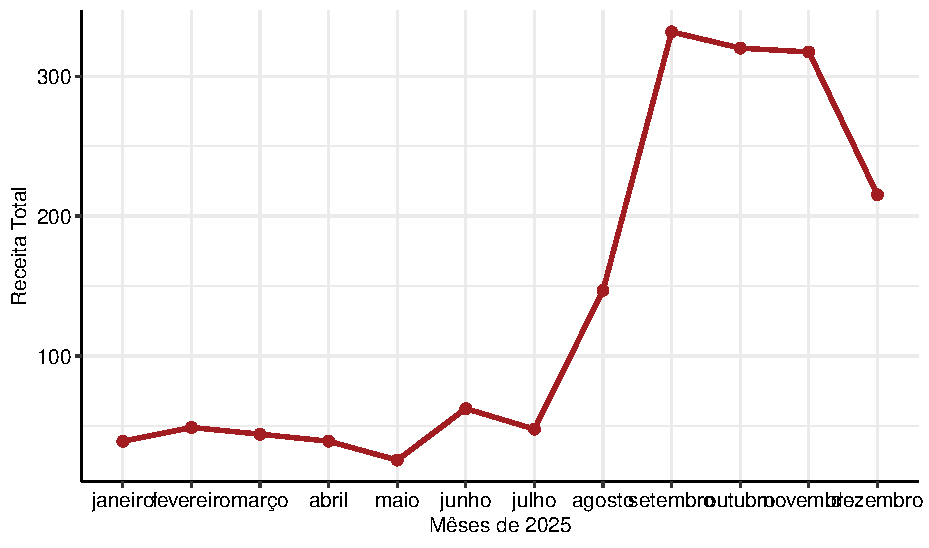
\includegraphics{entrega2_files/figure-pdf/fig-grafico2-1.pdf}

}

\end{figure}%

\begin{quadro}[H]

\caption{\label{quad-}Medidas resumo da}

\centering{

\begin{tabular} { | l |
            S[table-format = -Inf.2]
            |}
    \hline
        \textbf{Estatística} & \textbf{Valor} \\
        \hline
        Média & 136,53 \\
        Desvio Padrão & 124,89 \\
        Variância & 15597,14 \\
        Mínimo & 25,63 \\
        1º Quartil & 42,88 \\
        Mediana & 55,69 \\
        3º Quartil & 240,79 \\
        Máximo & 331,66 \\
    \hline
    \end{tabular}

}

\end{quadro}%




\end{document}
